\section{The index}
\label{sec:indice}

Partial delegation is the most common rating of a task, full delegation is rare, and the occupations at the top are clerical and administrative.

\subsection{Tasks}

Of the \cifra{cobertura.tareas.puntuadas} task statements with a valid consensus, \cifra{tareas.nivel0.pct}\% are rated L0, \cifra{tareas.nivel1.pct}\% L1, \cifra{tareas.nivel2.pct}\% L2 and \cifra{tareas.nivel3.pct}\% L3, so that \cifra{tareas.l2.pct}\% of statements reach at least partial delegation before any weighting.
L2 is the modal level.
Agents, as the models judge them, can execute substantial parts of many tasks but can finish very few of them without a human step.
Ties between models, resolved to the lower level as preregistered, affect \cifra{tareas.empates.pct}\% of tasks.
The two models agree with each other at Krippendorff's $\alpha$ = \cifra{agree.alpha.modelos} (ordinal) and at quadratic-weighted $\kappa$ = \cifra{agree.kappa.sonnet_haiku}.

\subsection{Occupations}

Table~\ref{tab:ocupaciones} lists the ten most and the ten least delegable of the \cifra{cobertura.isco} ISCO-08 unit groups covered by the crosswalk (\cifra{cobertura.isco.imputados} of them inherit the tasks of their parent group).
The index spans its whole range.
At the top, \cifra{extremo.isco.n.max} unit groups reach the maximum of \cifra{extremo.isco.top1.l2}\%; ranked within them by the share-based index, the first three are \cifra{extremo.isco.top1.nombre} (ISCO \cifra{extremo.isco.top1.id}); \cifra{extremo.isco.top2.nombre} (\cifra{extremo.isco.top2.id}); and \cifra{extremo.isco.top3.nombre} (\cifra{extremo.isco.top3.id}). The tied groups also include payroll clerks, accounting associate professionals, personnel clerks and database designers and administrators.
At the bottom, \cifra{extremo.isco.n.min} unit groups sit at the minimum of \cifra{extremo.isco.bot1.l2}\%, led, by the share-based index, by \cifra{extremo.isco.bot1.nombre} (\cifra{extremo.isco.bot1.id}); \cifra{extremo.isco.bot2.nombre} (\cifra{extremo.isco.bot2.id}); and \cifra{extremo.isco.bot3.nombre} (\cifra{extremo.isco.bot3.id}); the tied groups also include stonemasons, concrete placers, sewing and embroidery workers and shoemakers.
Full delegation is concentrated in a few clerical groups: coding and proof-reading clerks, typists and word processing operators, contact centre salespersons, receptionists and data entry clerks have the largest shares at L3.

Figure~\ref{fig:isco} aggregates unit groups to the nine major groups with implied world employment weights.
Managers reach \cifra{gg.1.l2}\%, professionals \cifra{gg.2.l2}\%, technicians and associate professionals \cifra{gg.3.l2}\% and clerical support workers \cifra{gg.4.l2}\%.
Service and sales workers sit in the middle at \cifra{gg.5.l2}\%.
The manual groups sit far below: \cifra{gg.6.l2}\% for skilled agricultural workers, \cifra{gg.7.l2}\% for craft and related trades, \cifra{gg.8.l2}\% for plant and machine operators and \cifra{gg.9.l2}\% for elementary occupations.
The order is the one exposure indices produce, with cognitive and office work on top and manual work at the bottom; Section~\ref{sec:validacion} quantifies how close it is.
Two features are specific to delegation.
Managers rank first at L2 or above but, like professionals, have very little weight at L3: the models leave the decision with a human.
Clerical support workers have by far the largest share at L3 of any major group, because their tasks are digital, specified by a goal and accepted by someone else.

% generado por analisis/tablas.py — no editar a mano
\begin{table}[t]
\centering\footnotesize
\caption{The ten most and ten least delegable ISCO-08 unit groups. ADI: task-weighted share at L2 or L3; ADI3: at L3; ADIs: weighted mean share of task time delegable, with 95\% bootstrap interval (1,000 draws, tasks resampled within occupation). \textbf{Synthetic placeholder values, not results.}}
\label{tab:ocupaciones}
\begin{tabular}{lp{5.6cm}rrrcr}
\toprule
ISCO & Unit group & ADI & ADI3 & ADIs & 95\% CI (ADIs) & Tasks \\
\midrule
\multicolumn{7}{l}{\emph{Most delegable}}\\
3342 & Legal secretaries & 94.5 & 33.7 & 67.6 & [59.5, 75.8] & 14 \\
4322 & Production clerks & 93.4 & 55.1 & 75.3 & [67.9, 82.3] & 17 \\
3252 & Medical records and health information technicians & 88.0 & 49.9 & 69.3 & [61.1, 76.0] & 33 \\
1311 & Agricultural and forestry production managers & 88.0 & 43.8 & 69.7 & [61.9, 76.6] & 30 \\
1312 & Aquaculture and fisheries production managers & 88.0 & 43.8 & 69.7 & [62.6, 76.2] & 30 \\
3352 & Government tax and excise officials & 87.5 & 14.1 & 64.1 & [57.9, 70.0] & 21 \\
1341 & Child care services managers & 87.4 & 42.6 & 68.1 & [59.7, 76.3] & 17 \\
2633 & Philosophers, historians and political scientists & 87.2 & 51.4 & 70.2 & [65.7, 75.2] & 57 \\
2631 & Economists & 86.8 & 33.6 & 68.2 & [62.7, 73.8] & 34 \\
1211 & Finance managers & 86.7 & 40.1 & 68.2 & [62.3, 74.2] & 39 \\
\midrule
\multicolumn{7}{l}{\emph{Least delegable}}\\
7215 & Riggers and cable splicers & 21.0 & 0.0 & 26.9 & [17.1, 37.6] & 14 \\
7213 & Sheet-metal workers & 19.9 & 9.8 & 29.0 & [21.3, 36.3] & 51 \\
7126 & Plumbers and pipe fitters & 19.2 & 5.6 & 24.8 & [17.6, 31.9] & 44 \\
7125 & Glaziers & 19.0 & 7.6 & 26.1 & [17.6, 35.2] & 27 \\
9111 & Domestic cleaners and helpers & 18.9 & 7.8 & 31.3 & [21.8, 41.9] & 20 \\
9112 & Cleaners and helpers in offices, hotels and other establishments & 17.9 & 4.5 & 28.2 & [22.2, 33.8] & 61 \\
5153 & Building caretakers & 17.4 & 6.4 & 28.0 & [19.1, 37.8] & 21 \\
9123 & Window cleaners & 17.4 & 6.4 & 28.0 & [19.1, 38.9] & 21 \\
9122 & Vehicle cleaners & 17.3 & 0.0 & 25.3 & [16.4, 35.4] & 20 \\
9129 & Other cleaning workers & 8.0 & 0.0 & 21.6 & [14.2, 29.9] & 22 \\
\bottomrule
\end{tabular}
\end{table}


\begin{figure}[t]
  \centering
  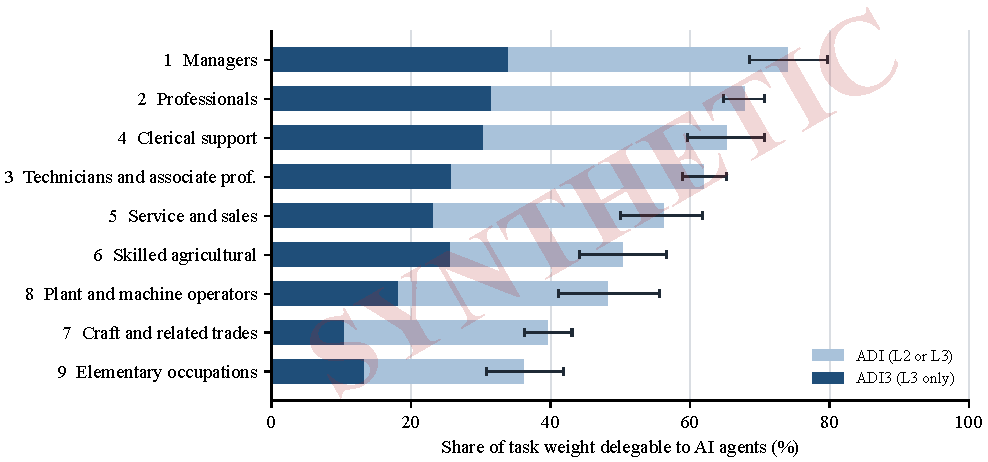
\includegraphics[width=0.92\linewidth]{fig/fig3_isco}
  \caption{ADI by ISCO-08 major group. Light bars: share of task weight at L2 or L3 (ADI); dark bars: share at L3 (ADI3). Whiskers: 95\% bootstrap interval of ADI (1,000 draws, tasks resampled within occupation). Unit groups are averaged with implied world employment weights. Generated by \texttt{analisis/figuras.py}.}
  \label{fig:isco}
\end{figure}

\subsection{Barriers}

Figure~\ref{fig:barreras} decomposes the task weight that each barrier flags by major group (exploratory).
Two barriers split the occupational structure.
The physical barrier flags most of the task weight in the five manual and service groups, from \cifra{gg.5.barrera_fisica.pct}\% in service and sales work to \cifra{gg.6.barrera_fisica.pct}\% in agriculture, \cifra{gg.7.barrera_fisica.pct}\% in crafts, \cifra{gg.8.barrera_fisica.pct}\% among operators and \cifra{gg.9.barrera_fisica.pct}\% in elementary occupations, and it is what keeps them low.
In the four office groups the most frequent flag is access, which marks between \cifra{gg.2.barrera_acceso.pct}\% (professionals) and \cifra{gg.1.barrera_acceso.pct}\% (managers) of task weight: the task depends on systems, data or places an agent would not normally reach.
Accountability is highest among professionals (\cifra{gg.2.barrera_responsabilidad.pct}\%), technicians (\cifra{gg.3.barrera_responsabilidad.pct}\%) and managers (\cifra{gg.1.barrera_responsabilidad.pct}\%), and trust among managers (\cifra{gg.1.barrera_confianza.pct}\%) and professionals (\cifra{gg.2.barrera_confianza.pct}\%), where tasks involve signatures, liability, persuasion and care; trust is also frequent in service and sales work (\cifra{gg.5.barrera_confianza.pct}\%).
Clerical work carries the fewest accountability flags of any group (\cifra{gg.4.barrera_responsabilidad.pct}\%) and few trust flags (\cifra{gg.4.barrera_confianza.pct}\%), which is why it is the group that reaches full delegation.
The barriers stack, so a task can carry several; the figure reports each one separately rather than assigning a single cause.

\begin{figure}[t]
  \centering
  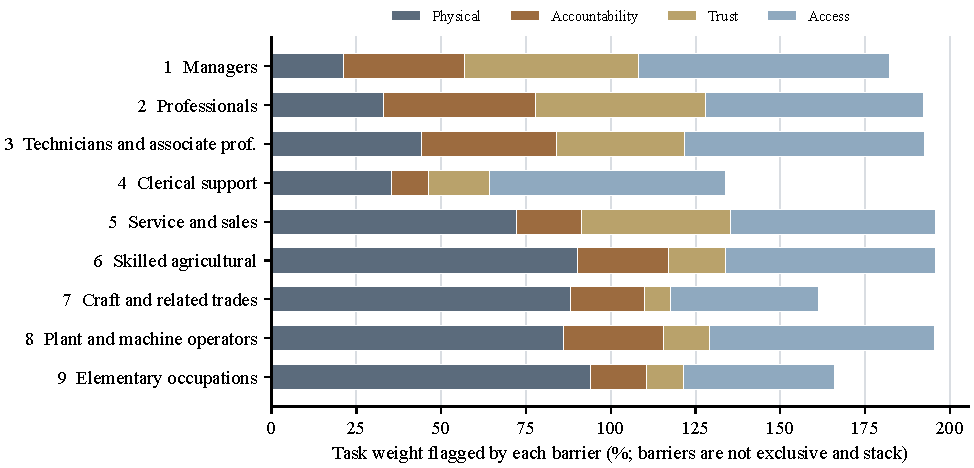
\includegraphics[width=0.92\linewidth]{fig/fig6_barreras}
  \caption{Barriers that keep tasks below full delegation, by ISCO-08 major group: task weight flagged by each barrier (fraction of models that flag it, weighted as in the index). Barriers are not mutually exclusive and stack. Generated by \texttt{analisis/figuras.py}.}
  \label{fig:barreras}
\end{figure}

\subsection{Task length (H4)}

H4 is supported: full delegation peaks for tasks that take a human about twelve minutes.
The probability that a task is fully delegable follows an inverted U in the log of the minutes a human needs for it: the logistic coefficients are \cifra{h4.b1} on log minutes (one-sided \pval{h4.p1}) and \cifra{h4.b2} on its square (\pval{h4.p2}), over \cifra{h4.n} tasks clustered in \cifra{h4.n.clusters} O*NET occupations.
The implied peak is at about \cifra{h4.pico.minutos} minutes of human work.
Very short tasks are often moments inside a physical or interpersonal activity, which an agent cannot isolate and finish on its own.
Long tasks bundle several steps, including judgement, coordination or sign-off, and one human step is enough to keep the whole task at L2.
Full delegation lives in between, in self-contained pieces of digital work.
The minutes are themselves a model estimate, recorded in the same call as the level, so the shape of the curve should be read as the models' view of task length rather than as a measured duration.

\subsection{Robustness}

The occupational index is not an artefact of the task-to-occupation assignment: the dispersion of $\mathrm{ADI}_o$ across unit groups (standard deviation \cifra{placebo.sd.obs}) compares with a mean of \cifra{placebo.sd.media} under the permutation null (\pval{placebo.p}).
With uniform task weights the world headline is \cifra{titular.global.l2.pesos_uniformes}\%, and without the imputed unit groups \cifra{titular.global.l2.sin_imputados}\%.

The choice of model matters more than any weighting choice.
Model by model, the world headline is \cifra{titular.modelo.sonnet.l2}\% with Sonnet and \cifra{titular.modelo.haiku.l2}\% with Haiku.
Haiku is the more generous rater: it places many more tasks at L2 or above.
Because the preregistered consensus takes the lower level when the two models disagree, the consensus headline of \cifra{titular.global.l2}\% stays close to Sonnet, the primary rater, and the gap to Haiku is a measure of how much the index depends on which model is asked.
Both models are stable across repeated calls (Section~\ref{sec:validacion}), so the difference is systematic, not noise.
